\chapter{Investigating Extract Method Refactoring Associated with Code Reuse}
\label{ChCibse}


\noindent\textit{Refactoring is a well-know technique that is frequently studied by the scientific community.
However, little is known about the actual reasons developers refactor.
In this study, we investigate the relationship between Extract Method refactoring and code reuse, in order to better understand the motivations behind it.
After analyzing over 10,000 revisions of 10 open source systems, we found evidence that, in 56.9\% of the cases, Extract Method is motivated by code reuse.
Also, in a small portion of these cases (7.9\%), reuse eliminates duplicate code that already exists in the system.
Finally, we also find that there are cases in which Extract Method favored long-term code reuse, even though their initial motivation were not code reuse.
}

\section{Introduction}


There is a common sense that refactoring effort is mainly driven by certain code patterns known as \emph{Bad Smells} ~\citep{Fowler:1999}, which signal system design problems. However, there are few empirical studies investigating the actual motivations behind refactoring, especially for those refactoring types that may serve multiple purposes.
%the motivation behind refactoring is an issue that is still little explored and
In particular, \emph{Extract Method}, one of the most widely applied refactorings in practice ~\citep{MurphyHill2012, negara2013}, serves multiple porposes.
For example, \cite{tsantalis_empiricalstudy} found nine distinct motivations for this refactoring, some of them related to the need for system extension rather than to code problems.

For this reason, this study investigates the relationship between Extract Method refactoring and code reuse.
We suspect that in many cases in which a method is extracted the developer intends to reuse code. For example, when adding a new feature, a developer may identify a code snippet in the system that shares common behavior with the new feature, extract such code as a new method, and reuse it.
Specifically, we investigate three research questions:

\begin{description}
\item[RQ1] How often is Extract Method motivated by code reuse?
\item[RQ2] How often is Extract Method motivated by removing duplicate code?
\item[RQ3] How often does Extract Method favors code reuse?% later, even though it was not initially motivated by code reuse?
\end{description}

We believe that answers to these questions can contribute to a better understanding of why development teams refactor their code. Such knowledge may be relevant to propose or improve techniques and methodologies employed in software development. In particular, it may be possible to refine existing tools specialized in recommending the Extract Method~\citep{Silva:2014, Tsantalis:2011} refactorings, as new heuristics can be developed to address the most frequently occurring scenarios in practice.

The remainder of this chapter is organized as follows. Section~\ref{smetodologia} describes the methodology used in this study.
Section~\ref{sresultados} presents the results obtained and answers the research questions raised.
%Section~\ref{srevisao} presents related works found in the literature.
Section~\ref{reusepatterns} formalizes and provides examples for the reuse patterns we found during the analysis.
Section~\ref{sameacas} discusses threats to the validity of the study.
Finally, Section~\ref{sconclusao} presents the conclusions.


\section{Methodology}
\label{smetodologia}

The methodology employed in this study, illustrated in Figure~\ref{ioverview}, can be divided into three steps:
\begin{enumerate}
\item We selected a set of Java repositories from GitHub using predefined criteria.
\item We detected \emph{Extract Method} refactorings applied to the systems with the aid of a tool. To this end, each code change (\emph{commit}) in the version history was analyzed.
\item We counted the number of invocations of the extracted methods along the version history. 
To this end, all future revisions were analyzed to identify method invocations, regardless of when they were introduced.
\end{enumerate}
In the following sections we describe the details of each step.

\begin{figure}[htbp]\centering
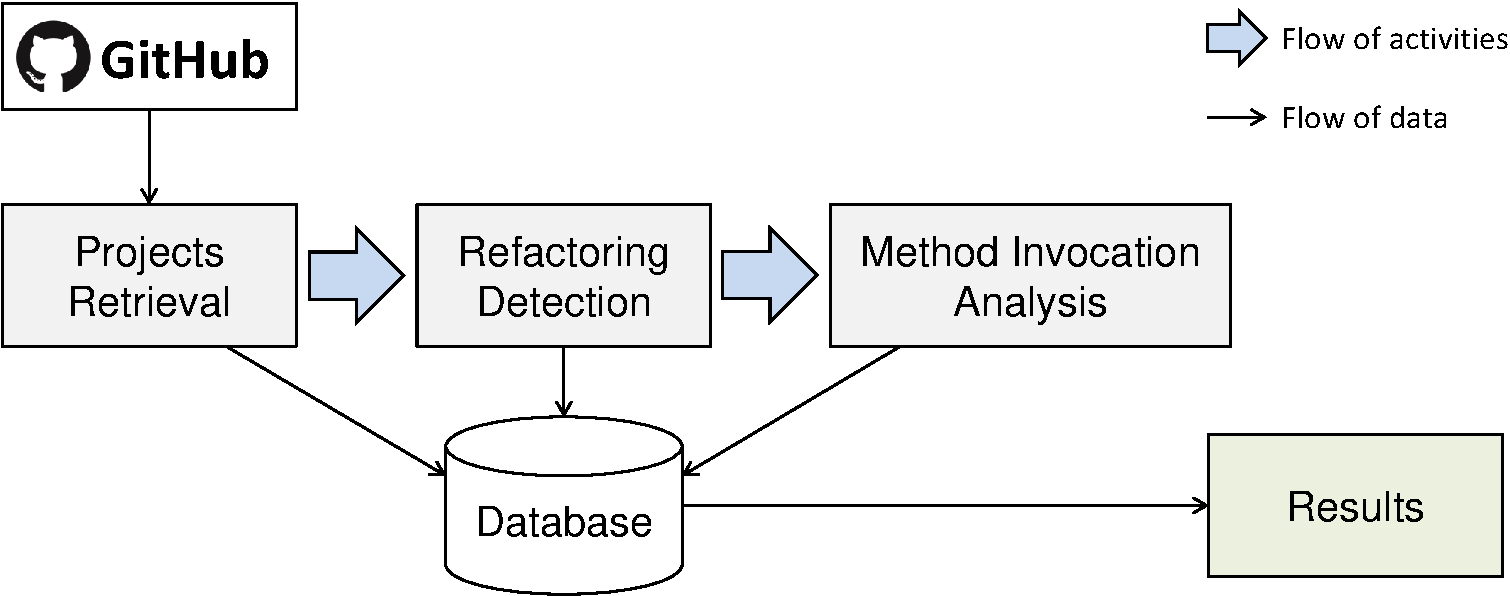
\includegraphics[width=0.8\textwidth]{img/ch5/overview-en.pdf}
\caption{Overview of the methodology}
\label{ioverview}
\end{figure}

\subsection{Selection of the Java repositories}
\label{ssystems}

To select the GitHub repositories, we defined the criteria listed below, according to good practices on mining GitHub repositories described in the literature~\citep{kalliamvakou2014promises}:
\begin{itemize}
\item Projects must have Java as the primary language, due to limitations of the tools used in the analysis.
\item Projects must have at least six months of development to avoid projects that have not gone through a relevant maintenance time.
\item Projects must have at least 200 revisions for the same reasons as the previous restriction.
\item Projects should not be derived (\emph{forks}) from another project to avoid duplicate data.
\item The projects obtained must be the 100 most popular projects that meet the other criteria, using the \texttt{stargazers\_count} field as a metric.
\end{itemize}


\begin{table}[bp]\centering
\renewcommand{\arraystretch}{1.3}
\caption{Studied repositories}
\begin{tabular}{@{}ll@{}}\toprule
Repository & Description \\
\midrule
android & GitHub Android App \\
android-async-http & An Asynchronous HTTP Library for Android \\
clojure & The Clojure programming language \\
facebook-android-sdk & SDK to integrate Android apps with Facebook Platform \\
jsoup & Java HTML Parser \\ %jquery
junit & A testing framework for Java. \\
picasso & A powerful image downloading and caching API for Android \\
spark & A Sinatra inspired framework for Java \\
storm & Distributed and fault-tolerant realtime computation system \\
yuicompressor & A JavaScript compressor \\
\bottomrule
\end{tabular}
\label{ch5:tsystems}
\end{table}

From the set of 100 repositories, we selected a random sample of 10 systems to perform this study due to limitations imposed by the long time required to perform the analysis on the complete data. Table~\ref{ch5:tsystems} lists the selected repositories and a brief description of each. Note that there are well-known projects among them, such as the JUnit testing framework and the Clojure programming language.

\subsection{Detecting refactorings}
\label{srefactoringdetection}

In this step, we analyzed each commit from the selected repositories to find instances of Extract Method refactoring. For this task, we used an automated approach to find refactorings proposed by \cite{tsantalis_empiricalstudy}, which we will denote as RefactoringMiner~0.1. Such approach compares the source code before and after a code change and employs a combination of heuristics designed to identify eleven types of refactoring.
In this study, our interest lies in Extract Method refactoring, whose detection heuristics are described below.

Let $M^+$ be the set of methods that were added between two consecutive revisions $v$ and $v'$. Additionally, let $M^=$ be the set of methods that exist both in $v$ and $v'$ (they were neither added or deleted between revisions).
A method $m_j$ is extracted from another method $m_i$ when four conditions are met:
\begin{itemize}
\item $m_i \in M^=$
\item $m_j \in M^+$
\item The body of $m_i$ before the change contains the statements within the body of $m_j$
\item The body of $m_i$ after the change contains an invocation of $m_j$
\end{itemize}
%Its important to note that the above conditions can be met for more then one pair 
If the above conditions are met for more than one pair $(m_i, m_j)$ for the same $m_j$, this means that the method was extracted from more than one location.
For example, if these conditions hold for two pairs $(m_1, m_2)$ and $(m_3, m_2)$, then the code encapsulated by $m_2$ was duplicated in $m_1$ and $m_3$.

We executed the aforementioned heuristic comparing each pair of consecutive revisions, covering the entire commit history of each repository.
We only discarded commits that merge changes from different branches, because otherwise we would collect duplicate information. For example, suppose a developer applies a refactoring $r_1$ in a branch $b_1$. When the developer merges $b_1$ with $b_2$, the merge commit will apply the refactoring in $b_2$ too.
We also modified the source code of the original tool to automate the navigation in the commit graph of a repository. Finally, we modified its source code to prevent it from compiling the entire project during its analysis. This optimization allowed us to reduce the execution time significantly and made it possible to use it in large scale.


\subsection{Counting the method invocations}
\label{sinvocationcount}

To detect the number of invocations of the methods of interest, we developed a tool based on the JDT Core API, which is the API used by the Eclipse IDE to parse and manipulate Java code. This API allows us to analyze the source code at the Abstract Syntactic Tree (AST) level, making it possible to find every method invocation in the code. In addition, the JDT Core API provides a resolution mechanism to bind a method invocation to its declaration.

Taking advantage of information provided by such API, we searched for invocations of each method of interest in each revision of the system. Specifically, the methods of interest were the ones that were extracted from another method at some point in the history, i.e,. they were created by applying an Extract Method refactoring.
For that reason, invocations of methods defined externally to the project, i.e., methods defined in third party APIs, are not relevant to the analysis.
This makes it possible to use JDT Core API even in the absence of all build dependencies of the project.
By the end of this step, we recorded the number of invocations of each extracted method, along with the methods that invoked them. This information is recorded for every revision after the extracted method is introduced. 



\section{Results}
\label{sresultados}

\begin{table}[b]\centering
\renewcommand{\arraystretch}{1.3}
\caption{Statistics from the analyzed repositories}
\begin{tabular}{@{}lrrr@{}}\toprule
Repository & Commits & Analyzed Methods & Extracted Methods \\
\midrule
android & 2,351 & 3,386 & 100 (3.0\%) \\
android\-async\-http & 557 & 726 & 34 (4.7\%) \\
clojure & 2,629 & 6,276 & 122 (1.9\%) \\
facebook-android-sdk & 451 & 4,840 & 144 (3.0\%) \\
jsoup & 711 & 1,760 & 35 (2.0\%) \\
junit & 1,611 & 5,822 & 107 (1.8\%) \\
picasso & 461 & 1,357 & 41 (3.0\%) \\
spark & 281 & 738 & 19 (2.6\%) \\
storm & 1,491 & 4,987 & 38 (0.8\%) \\
yuicompressor & 388 & 269 & 9 (3.3\%) \\
\midrule
Total & 10,931 & 30,161 & 649 (2.2\%) \\
\bottomrule
\end{tabular}
\label{tcommits}
\end{table}

In this section we present and discuss the results of the analysis. In total, we analyzed 10,931 commits from 10 repositories, as detailed in Table~\ref{tcommits}.
Additionally, Table~\ref{tcommits} presents the number of distinct methods declared along the history of each repository and the number of methods created by applying Extract Method.
Interestingly, 649 methods out of 30,161 are extracted, which corresponds to 2.2\%. Moreover, every repository contains extracted methods.
It is important to note that the number of methods analyzed is always greater than or equal to the total number of methods in the last version of a system. That is because throughout the evolution of the system, methods are created and removed. In fact, out of 30,161 methods analyzed, only 17,707 (58.7\%) of them exist in the last version of their respective projects.
In the next sections we discuss each research question in detail, taking into consideration the set of 649 extracted methods.

\subsection{RQ1: How often is Extract Method motivated by code reuse?}
\label{study1:rq1}

\begin{table}[b]\centering
\renewcommand{\arraystretch}{1.3}
\caption{Extract Method instances related to code reuse}
\begin{tabular}{@{}lrrr@{}}\toprule
Repository & Extracted methods & Invocations $\geq 2$ & Duplicated code\\
\midrule
android & 100 & 60 (60.0\%) & 10 (10.0\%) \\
android\-async\-http & 34 & 15 (44.1\%) & 3 (8.8\%) \\
clojure & 122 & 72 (59.0\%) & 11 (9.0\%) \\
facebook\-android\-sdk & 144 & 95 (66.0\%) & 9 (6.3\%) \\
jsoup & 35 & 24 (68.6\%) & 1 (2.9\%) \\
junit & 107 & 44 (41.1\%) & 11 (10.3\%) \\
picasso & 41 & 26 (63.4\%) & 4 (9.8\%) \\
spark & 19 & 10 (52.6\%) & 1 (5.3\%) \\
storm & 38 & 18 (47.4\%) & 0 (0.0\%) \\
yuicompressor & 9 & 5 (55.6\%) & 1 (11.1\%) \\
\midrule
Total & 649 & 369 (56.9\%) & 51 (7.9\%) \\
\bottomrule
\end{tabular}
\label{treuse}
\end{table}


To answer this first research question, we searched for the following scenario: in a single commit, a developer extracts a method and invokes it two or more times in the system. We assume that, in such cases, the developer extracted the method to reuse it.
The second column of Table~\ref{treuse} presents the number of extracted methods that are reused (i.e., two or more invocations).
%In total 369 out of 649 methods fall in this scenario (56.9\%).
When analyzing each repository individually, we note that the lowest percentage of reused methods is 41.1\%, for \textit{junit} repository, and the highest percentage is 68.6\%, for \textit{jsoup}. Moreover, for 7 out of 10 repositories, the percentage of reused methods is above 50\%.
Last, 369 out of 649 methods fall in this scenario~(56.9\%), which yields the following answer to RQ1: \textbf{in~56.9\% of the cases developers apply Extract Method to reuse code}.


\subsection{RQ2: How often is Extract Method motivated by removing duplicate code?}


In this second research question, we investigate a more specific scenario: in a single commit, a developer extracts a method from two or more places of the system. As a consequence, duplicate code in the original methods is removed and replaced by invocations of the extracted method.
The last column of Table~\ref{treuse} shows how often such scenario occurs in total and in each repository.
We found at least one case of removal of duplicated code in each repository, except for the \textit{storm} project. The project with more occurrences is \textit{junit}, with 11 instances, which represents 10.3\% of all Extract Method instances. 
It is worth noting that such duplicate code removal scenario is a specialization of the scenario studied in RQ1.
That is, out of 369 methods extracted with more than one invocation, 51 were characterized as duplicate code removal.
In summary, we found the following answer to RQ2:  \textbf{in~7.9\% of the cases developers apply Extract Method to eliminate duplicate code in the system.} Although this case is less frequent than the prior, it could be observed in almost all repositories.


\subsection{RQ3: How often does Extract Method favor code reuse?}

\begin{table}[htbp]\centering
\renewcommand{\arraystretch}{1.3}
\caption{Extracted methods that were reused along the version history}
\begin{tabular}{@{}lrrr@{}}\toprule
Repository & Reused immediately & Reused later & Never reused\\
\midrule
android & 60 (60.0\%) & 3 (3.0\%) & 37 (37.0\%) \\
android-async-http & 15 (44.1\%) & 5 (14.7\%) & 14 (41.2\%) \\
clojure & 72 (59.0\%) & 5 (4.1\%) & 45 (36.9\%) \\
facebook-android-sdk & 95 (66.0\%) & 2 (1.4\%) & 47 (32.6\%) \\
jsoup & 24 (68.6\%) & 2 (5.7\%) & 9 (25.7\%) \\
junit & 44 (41.1\%) & 9 (8.4\%) & 54 (50.5\%) \\
picasso & 26 (63.4\%) & 2 (4.9\%) & 13 (31.7\%) \\
spark & 10 (52.6\%) & 2 (10.5\%) & 7 (36.8\%) \\
storm & 18 (47.4\%) & 1 (2.6\%) & 19 (50.0\%) \\
yuicompressor & 5 (55.6\%) & 0 (0.0\%) & 4 (44.4\%) \\
\midrule
Total & 369 (56.9\%) & 31 (4.8\%) & 249 (38.4\%) \\
\bottomrule
\end{tabular}
\label{treusetime}
\end{table}


While in the previous research questions we analyzed scenarios in which a method is extracted and reused in the same commit, this time we investigate whether extracted methods with a single invocation are eventually invoked by two or more methods throughout the evolution of the system. 
% In this case, we assume that the original intention of the Extract Method refactoring is not code reuse. , in such cases, the developer extracted the method to reuse it.
Table~\ref{treusetime} presents the number of methods that fall into this scenario (column~3), in contrast to the ones that already started with more than one invocation (column~2) and those that are never reused by other methods along the version history (column~4). The overall result shows that the extracted methods are reused later in 31 out of 649 cases (4.8\%). This scenario is observed in almost all repositories, except for the \textit{yuicompressor} (possibly because of the small number of extracted methods identified in it).
Table~\ref{treusetime} also shows that in 249 out of 649 cases (38.4\%) there is only one invocation of the extracted method throughout the entire history of the project, i.e., the method is never reused.
These results suggest the following answer to RQ3: \textbf{in 4.8\% of the cases that developers apply Extract Method, there is no initial intention to reuse code, but a reuse opportunity appeared later.} Although not frequent, this case is also consistently observed.


\section{Reuse patterns related to Extract Method}
\label{reusepatterns}



In the light of the results presented in previous sections, we propose three distinct patterns of code reuse associated with Extract Method refactoring:
%, which we denote by: \textit{Duplication}, \textit{Immediate Reuse}, and \textit{Later Reuse}.
\begin{description}
\item[Duplication:] In this scenario, a developer identifies duplicated code in two or more places in the system and applies Extract Method to fix the issue, replacing the duplicated code with a method invocation.
Therefore, the refactoring is applied to fix the \emph{Duplicated Code} bad smell, which is a classical motivation for Extract Method, as documented in the refactoring literature~\citep{Fowler:1999}.
Figure~\ref{iexdup} presents an example of this scenario in \textit{junit} project. A developer extracted the method \texttt{createLoader}, encapsulating a piece of duplicated code in methods \texttt{load} (lines~8--9) and \texttt{reload} (lines~12--13).
These lines of code, which were responsible for instantiating the \texttt{TestCaseClassLoader} class, are then replaced by the invocation of \texttt{createLoader}. It is interesting to note that a new statement was also introduced in \texttt{createLoader} (line~18), which would result in one more duplicate line of code if the method was not extracted.

% https://github.com/junit-team/junit/commit/ebe724e4b925fca5c9aeb6f7e282a5f0ae132232?diff=split
\begin{figure}[htbp]\centering
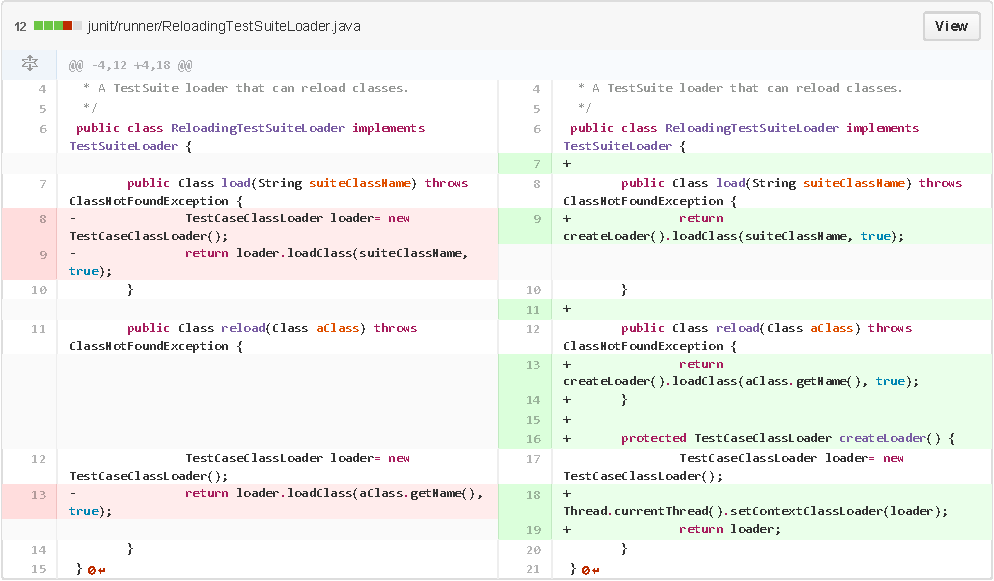
\includegraphics[width=1\textwidth]{img/ch5/dup.pdf}
\caption{Example of the \textit{Duplication} scenario}
\label{iexdup}
\end{figure}  


\item[Immediate Reuse:] In this scenario, a developer identifies the opportunity to reuse existing code when modifying the system, either to introduce new functionality or fix a problem. Extract Method is then applied and the new method is invoked in the new feature.
Figure~\ref{iexinit} presents an example of this scenario in the \textit{storm} project. A developer introduced a new method \texttt{tryPublish}, whose behavior was very similar to the existing \texttt{publish} method. To do this, an overloaded method \texttt{publish(Object, boolean)} was extracted from \texttt{publish(Object)} and reused in \texttt{tryPublish}. Note that the boolean parameter introduced in the extracted method allows a slight variation in the logic, enabling its reuse in both cases.
%It is interesting to note that in this scenario the developer prepares the system to receive the code he intends to introduce, avoiding code duplication, while in the previous scenario the developer solves an existing duplication problem.

% https://github.com/nathanmarz/storm/commit/1a9dca46abe4c937e6b5874a9d1b178163a95af4?diff=split

\begin{figure}[htbp]\centering
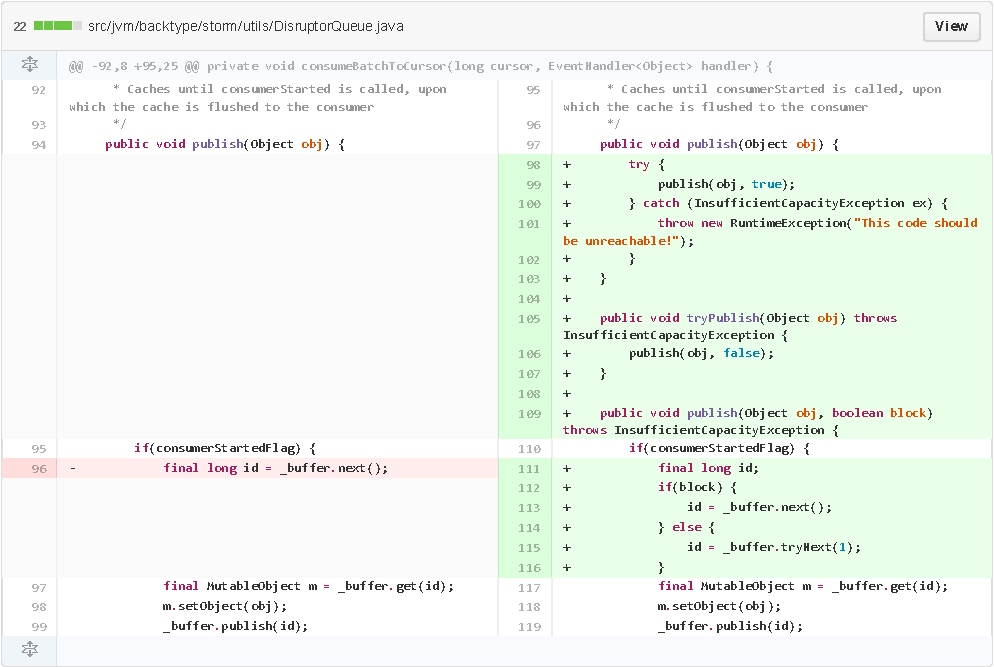
\includegraphics[width=1\textwidth]{img/ch5/init.pdf}
\caption{Example of the \textit{Immediate Reuse} scenario}
\label{iexinit}
\end{figure}


\item[Later Reuse:] In this scenario, a developer applies the Extract Method refactoring and the extracted method is invoked in only one location. However, in future code changes, a developer finds the opportunity to reuse that method. Therefore, there is no evidence that the initial motivation for the refactoring is code reuse, but it favors reuse later, possibly as a side effect.
Figure~\ref{iexpost} presents an example of this scenario in the \textit{clojure} project. A developer extracted the \texttt{isMacro} method from \texttt{analyzeSeq}, encapsulating the code between lines 2799--2805. In this case, the method was probably refactored to improve readability, since much of the logic in \texttt{analyzeSeq} was intended to determine whether a certain object is a macro, which became clearly indicated by the name of the extracted method. However, in a later modification, the same logic was required and another invocation of the \texttt{isMacro} method was introduced.
\end{description}

% https://github.com/loopj/android-async-http/commit/a947934ce9228579d34af082fa1bce577d728c25?diff=split
\begin{figure}[htbp]\centering
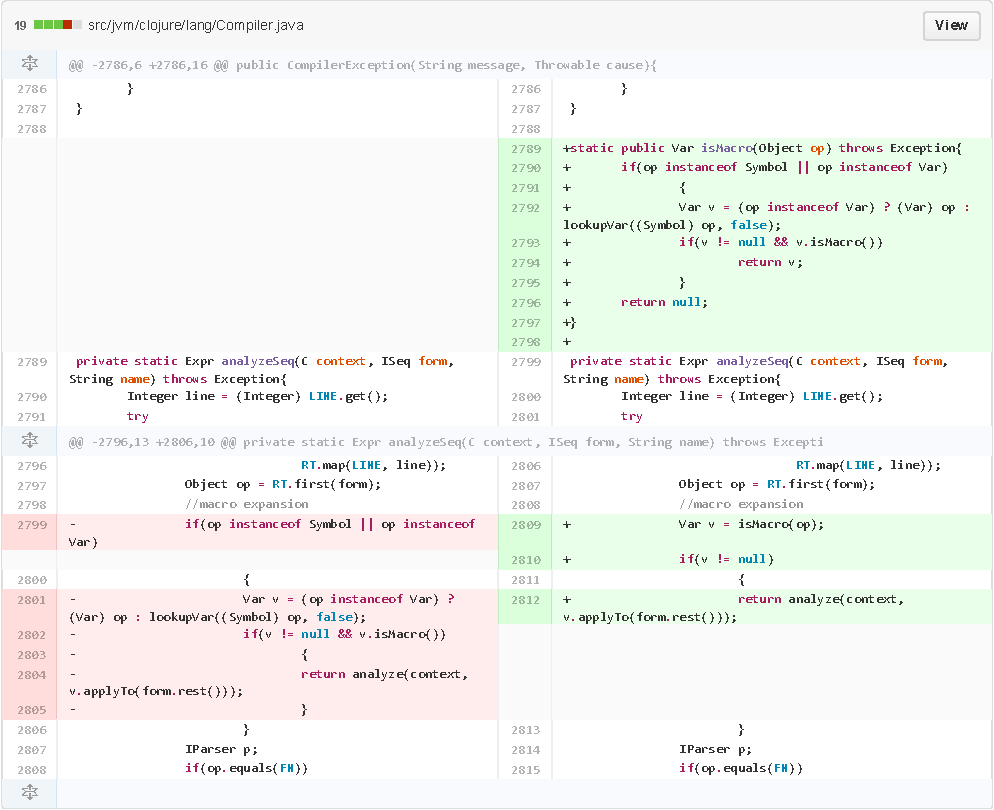
\includegraphics[width=1\textwidth]{img/ch5/post.pdf}
\caption{Example of the \textit{Later Reuse} scenario}
\label{iexpost}
\end{figure}



Figure \ref{ireuse} shows the proportion of the three observed reuse pattern in the studied repositories. Overall, the sum of the three scenarios represents 61.6\% of Extract Method instances, which indicates that code reuse is an important driver for refactoring effort. The complementary 38.4\% are those cases where the extracted methods are never reused.

\begin{figure}[htbp]\centering
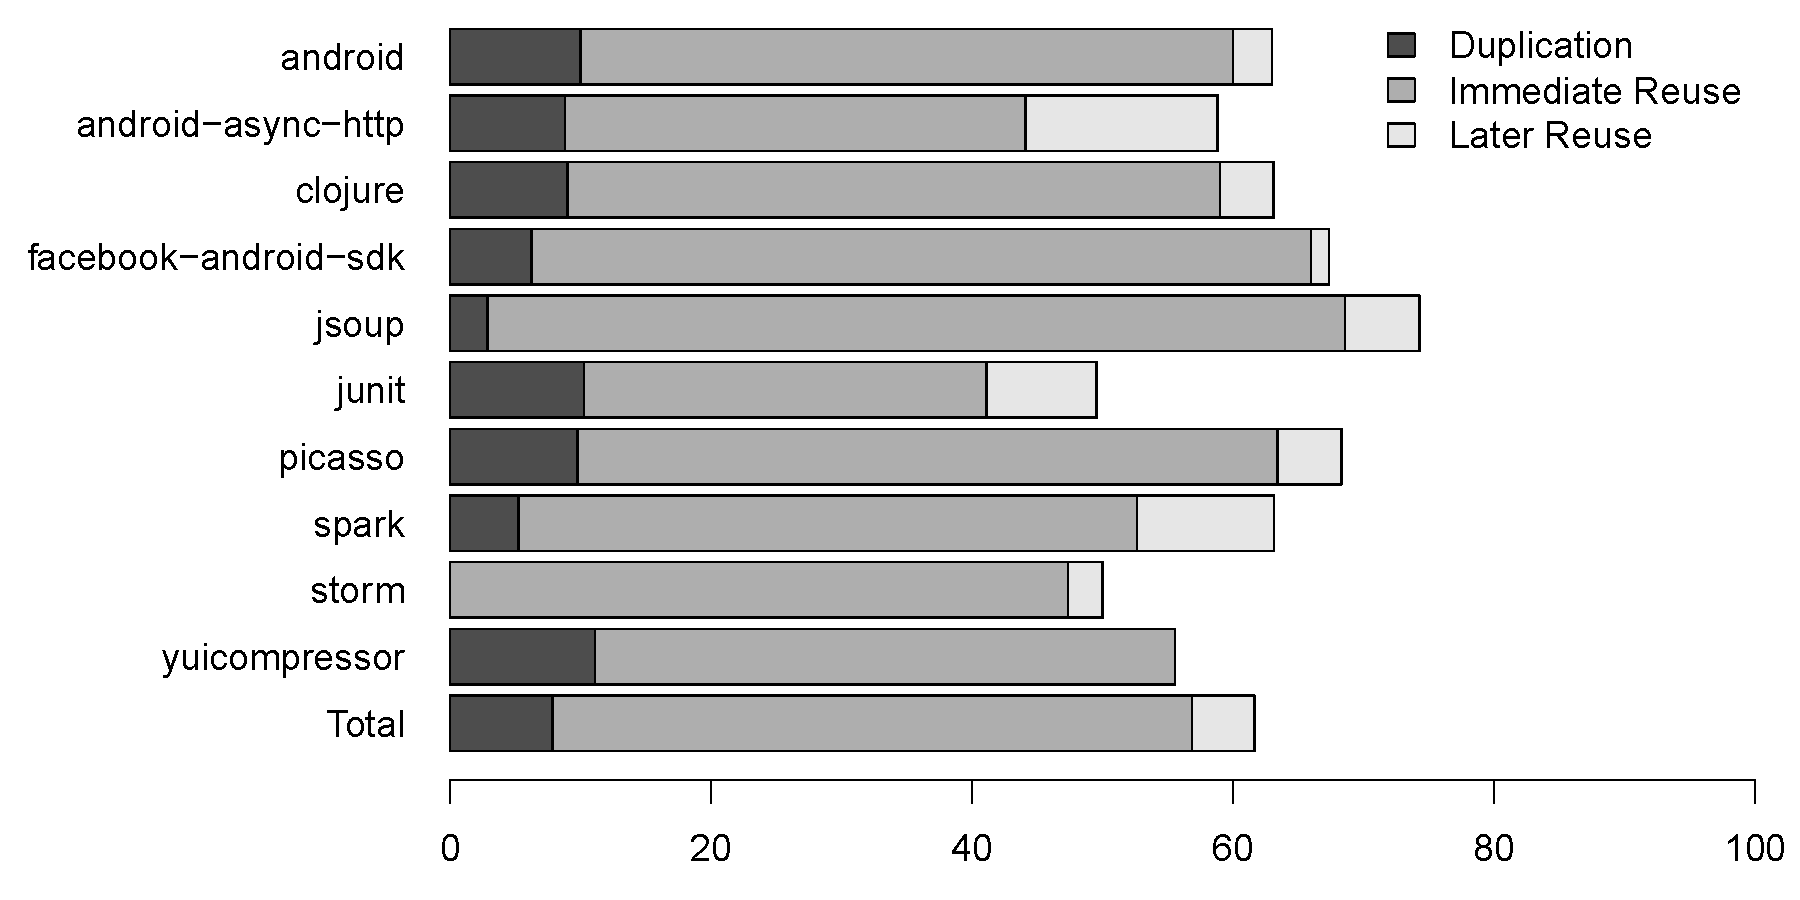
\includegraphics[width=1\textwidth]{img/ch5/barchart2.pdf}
\caption{Proportion of observed reuse patterns}
\label{ireuse}
\end{figure}


\section{Threats to Validity}
\label{sameacas}

There are at least two threats to the internal validity of the study:
\begin{itemize}
\item The accuracy of the results depends on how accurate the refactoring detection tool is. Although the authors reported a precision of  96.4\%~\citep{tsantalis_empiricalstudy}, precision could be different under the circumstances of this study.
To mitigate such a threat, we manually inspected a sample of the Extract Method instances we found. We choose 50 instances at random for manual inspection and assessed that 4 of them were false positives (92.0\% of precision).
Additionally, there is the possibility that the tool does not detect all Extract Method instances applied (false negatives). Unfortunately, it is not feasible to assess the tool recall by manually inspecting the code changes.

\item The validity of the results depends on the correctness of the method invocation analysis tooling developed specifically for this study. In fact, we believe that not every method invocation is identified for three reasons: (i) the methodology uses only static analysis and it is not able to identify method invocations relying on meta-programming features of the Java language, (ii) the JDT Core API is not able to resolve method invocation bindings in 100\% of the cases in the absence of the complete compilation dependencies, and (iii) extracted methods that are moved or renamed in a subsequent revision are not accounted for in the \emph{later reuse} scenario.
Nevertheless, such issues would only result in an underestimation of the number of invocations. Therefore, the existence of false negatives would not undermine the finding that code reuse is a major motivation for Extract Method.
\end{itemize}

We should also mention the threat of external validity, especially considering that the selected systems share the following characteristics:
\begin {itemize}
\item Only Java systems were considered, due to limitations of the analysis tools. The results may differ if we consider other programming languages.

\item The systems analyzed are all open source systems from a single source (GitHub). Results may differ for proprietary systems developed in a different context.
\end{itemize}

%\section{Related Work}
%\label{srevisao}

\section{Conclusion}
\label{sconclusao}

In this study we analyzed 10,931 commits from 10 open-source Java projects to investigate the relationship between Extract Method refactoring and code reuse. We found evidence that 56.9\% of the Extract Method instances are motivated by code reuse. Specifically, this occurs in two distinct scenarios: \textbf{Duplication} (7.9\% of cases) and \textbf{Immediate Reuse} (49.0\% of cases).
In addition, we found a third scenario, \textbf{Later Reuse}, in which Extract Method refactoring favored long-term code reuse, even though there was no indication that this was the initial intention (4.8\% of cases).
All three scenarios were found in virtually all systems analyzed in similar proportion.

The results obtained indicate that it is incorrect to assume that Extract Method refactoring is always associated with the resolution of an existing bad smell, such as \emph{Long Method} or \emph{Duplicated Code}. Approximately half of the cases analyzed fall into the \textbf{Immediate Reuse} scenario, in which a developer refactors existing code to enable code reuse in new code he is working on when modifying the system.
From another perspective, this also suggests that developers avoid introducing duplication when fixing a defect or implementing new functionality.

In particular, this observation has two implications for research on Extract Method recommendation approaches. First, regardless of the recommendation heuristic used, certain decisions made by a developer take into consideration the feature she will introduce to the system. Thus, it is quite challenging for a recommendation tool that relies only on the existing code to suggest an appropriate recommendation in these cases.
%Therefore, this should be taken into account when evaluating the precision of a heuristic.
Second, given that code reuse is a frequent scenario, new recommendation approaches could be explored, for example, suggesting the extraction of code snippets that are likely to be reused in the project.
